\documentclass{beamer}
\usepackage[latin1]{inputenc}
\usepackage{hyperref}
\usepackage{colortbl}
\usepackage{alltt}
%\usepackage{amsmath,amssymb, latexsym}
\usepackage{stmaryrd}
\usetheme{Warsaw}
\title[Termination Analysis Using Bitvector Arithmetic]{Termination Analysis of Imperative Programs Using Bitvector Arithmetic}
\author{Stephan Falke\inst{1}, Deepak Kapur\inst{2}, and Carsten Sinz\inst{1}}
\institute{\inst{1} Institute for Theoretical Computer Science, KIT, Germany \and %
  \inst{2} Dept. of Computer Science, University of New Mexico, USA}
\date{\footnotesize Verified Software: Theories, Tools, Experiments \\ VSTTE 2012}

\AtBeginSection[]
{
  \begin{frame}<beamer>
    \frametitle{Outline}
    \tableofcontents[currentsection,currentsubsection]
  \end{frame}
}

\makeatletter
% add a macro that saves its argument
\newcommand{\footlineextra}[1]{\gdef\insertfootlineextra{#1}}
\newbox\footlineextrabox

% add a beamer template that sets the saved argument in a box.
% The * means that the beamer font and color "footline extra" are automatically added. 
\defbeamertemplate*{footline extra}{default}{
    \begin{beamercolorbox}[ht=2.25ex,dp=1ex,leftskip=\Gm@lmargin]{footline extra}
    \insertfootlineextra
    %\par\vspace{2.5pt}
    \end{beamercolorbox}
}

\addtobeamertemplate{footline}{%
    % set the box with the extra footline material but make it add no vertical space
    \setbox\footlineextrabox=\vbox{\usebeamertemplate*{footline extra}}
    \vskip -\ht\footlineextrabox
    \vskip -\dp\footlineextrabox
    \box\footlineextrabox%
}
{}

% patch \begin{frame} to reset the footline extra material
\let\beamer@original@frame=\frame
\def\frame{\gdef\insertfootlineextra{}\beamer@original@frame}
\footlineextra{}
\makeatother

\setbeamercolor{footline extra}{fg=structure.fg}% for instance

\begin{document}

\begin{frame}
\titlepage
\end{frame}

\begin{frame}{Summary}
This paper proposes a novel method for \textcolor{red}{encoding the wrap-around
  behavior of bitvector arithmetic within integer arithmetic}, such
that existing methods for reasoning about the termination of integer
arithmetic programs can be employed for reasoning about the
termination of bitvector arithmetic programs.

\end{frame}
  
\begin{frame}{Outline}
\tableofcontents
\end{frame}

\section{Introduction}

\begin{frame}[fragile]{Existing Methods}
  Bitvectors are treated as (unbounded) integers (or as real numbers).

\medskip
  This approximation can cause errors in both directions:

\begin{itemize}

\begin{columns}
  \begin{column}{4.5cm}
\item Terminating wrt bitvector arithmetic, but non-terminating wrt
  integer arithmetic.

\begin{exampleblock}{Example}
\begin{verbatim}
void f(int i) {
  while (i > 0)  
    i++;
}
\end{verbatim}
\end{exampleblock}
    
\end{column}

\begin{column}{4.5cm}
\item Terminating wrt integer arithmetic, but non-terminating wrt
  bitvector arithmetic.

\begin{exampleblock}{Example}
\begin{verbatim}
void g(int i, int j) {
  while (i <= j) 
    i++;
}
\end{verbatim}
\end{exampleblock}

\end{column}
\end{columns}

\end{itemize}

\end{frame}

\begin{frame}{Related Work [CKR+10]}
Main differences:
\begin{itemize}
\item The use of quantifiers. Quantifier elimination before ranking
  function synthesis is expensive.
\item Template matching for linear ranking functions allows to use
  SAT, QBF and SMT solver.
\end{itemize}

\footlineextra{[CKR+10] Byron Cook, Daniel Kroening, Philipp R�mmer,
  Christoph M. Wintersteiger: Ranking Function Synthesis for
  Bit-Vector Relations. TACAS 2010: 236-250}
\end{frame}

\section{Termination Analysis in \texttt{KITTeL}}

\begin{frame}{The Approach of \texttt{KITTeL}}
\texttt{KITTeL} is a termination analysis tool on LLVM-IR.

\begin{block}{Bird's-eye view of \texttt{KITTeL}'s approach}
\begin{figure}
  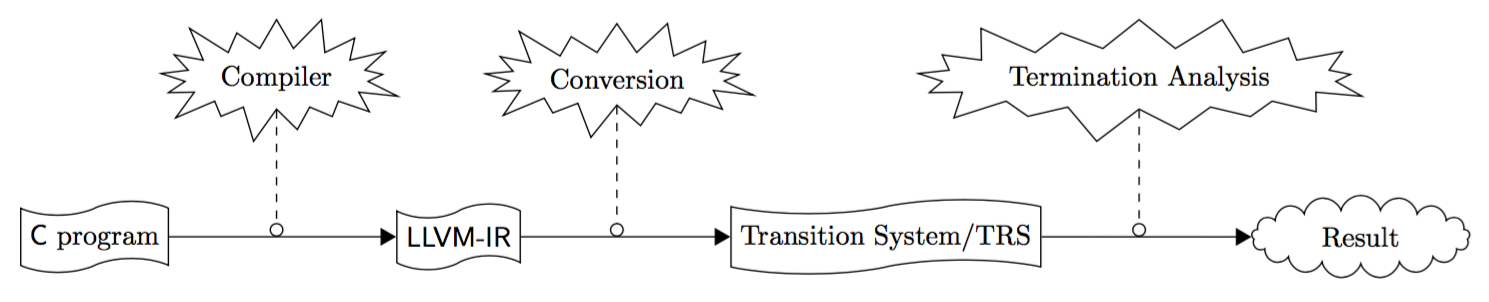
\includegraphics[width=\textwidth]{view.png}
\end{figure}
\end{block}

\end{frame}

\begin{frame}{From C to LLVM-IR}
From C code to LLVM-IR code, and then \emph{basic block graph}:
\begin{exampleblock}{Example 1}
\begin{figure}
  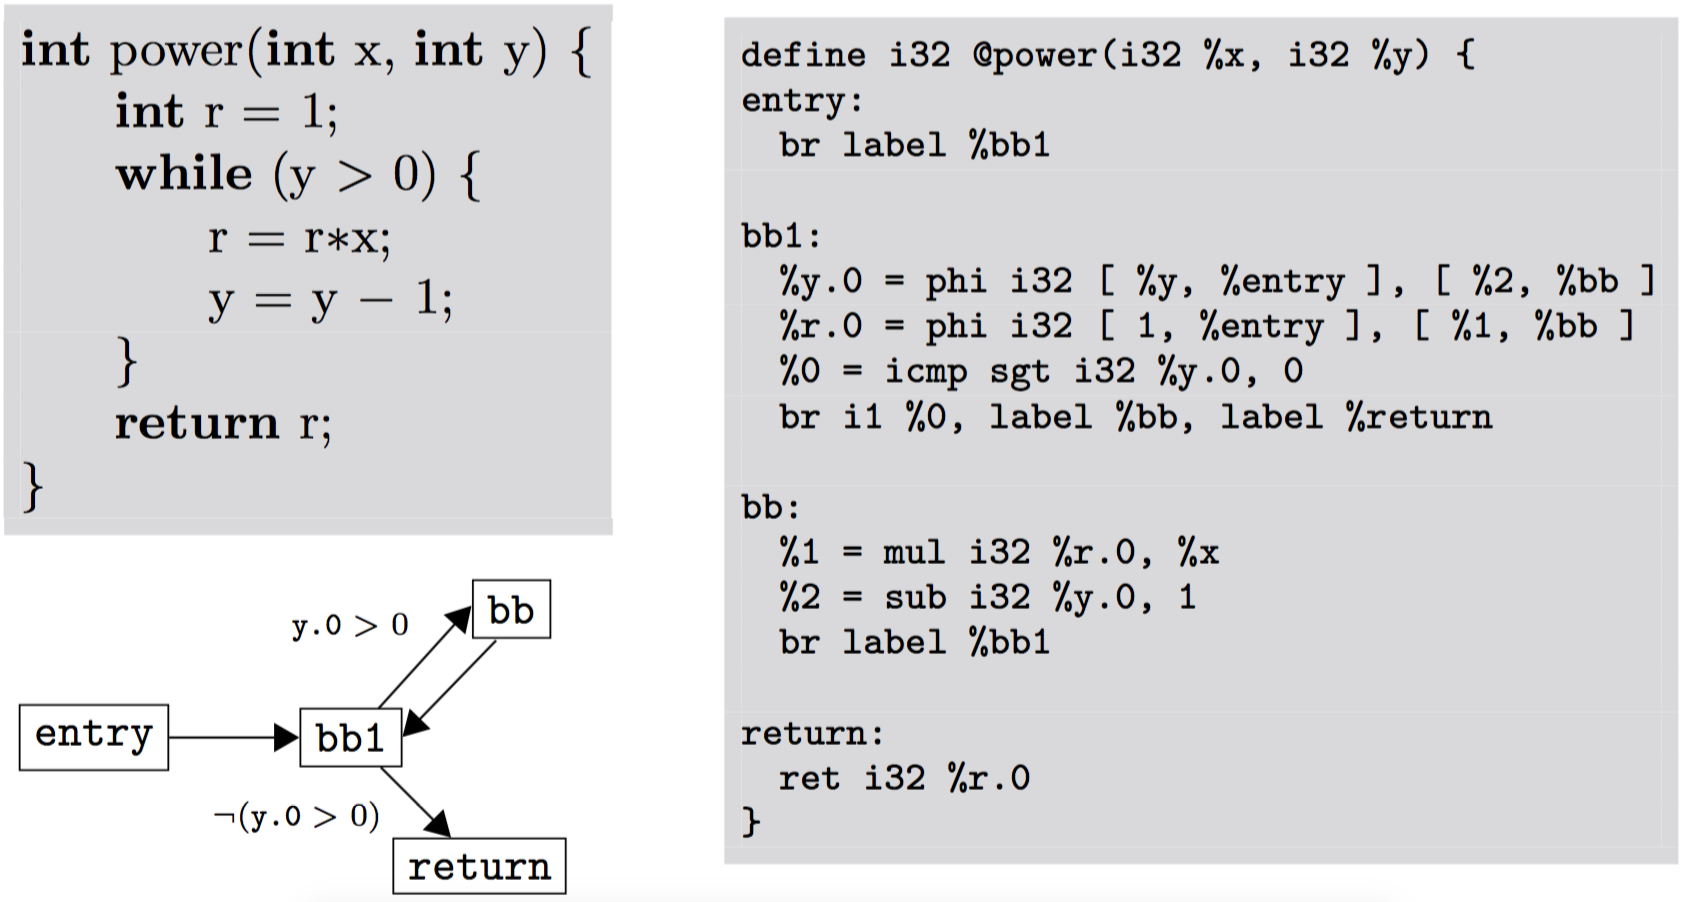
\includegraphics[width=\textwidth]{CtoLLVM.png}
\end{figure}
\end{exampleblock}
\end{frame}

\begin{frame}{From LLVM-IR to Transition System}
The corresponding transition system of Example~1:
\begin{exampleblock}{Example 1}
\begin{figure}
  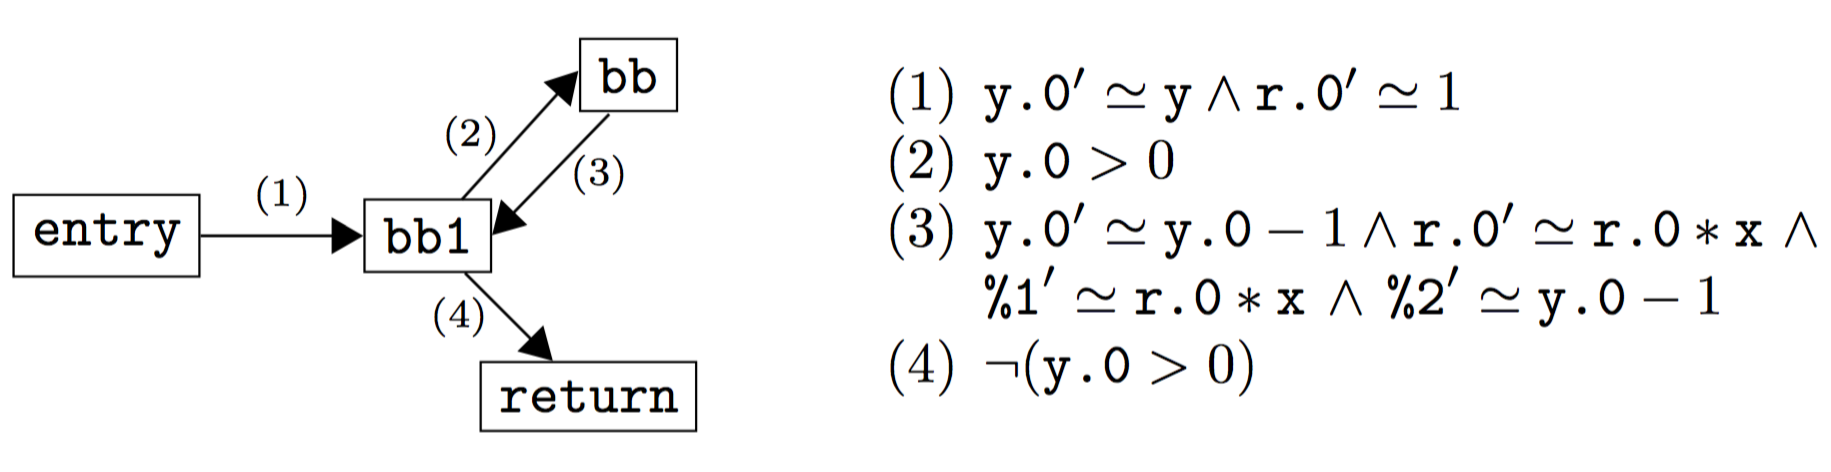
\includegraphics[width=\textwidth]{LLVMtoTS.png}
\end{figure}
\end{exampleblock}
\end{frame}

\begin{frame}[fragile]{From Transition Systems to TRSs}
\begin{itemize}
\item A transition system can be represented in the form of an
  \texttt{int}-based TRS.
\item Each transition $s_1 \rightarrow^\lambda s_2$ gives rise to a
  rewrite rule
\begin{center}
$s_1(x_1,\ldots,x_n) \rightarrow s_2(e_1,\ldots,e_n) ~ \llbracket\varphi\rrbracket$
\end{center}
\end{itemize}
\begin{exampleblock}{TRS of Example 1}
\footnotesize
\begin{tabular}{rcl}
$\verb|entry|(\verb|x|, \verb|y|, \verb|y.0|, \verb|r.0|, \verb|%1|, \verb|%2|)$ 
  & $\!\!\!\!\rightarrow\!\!\!\!$ 
  & $\verb|bb1|(\verb|x|, \verb|y|, \verb|y|, 1, \verb|%1|, \verb|%2|)$ \\
$\verb|bb1|(\verb|x|, \verb|y|, \verb|y.0|, \verb|r.0|, \verb|%1|, \verb|%2|)$ 
  & $\!\!\!\!\rightarrow\!\!\!\!$ 
  & $\verb|bb|(\verb|x|, \verb|y|, \verb|y.0|, \verb|r.0|, \verb|%1|, \verb|%2|) 
  ~ \llbracket \verb|y.0| > 0 \rrbracket$ \\
$\verb|bb1|(\verb|x|, \verb|y|, \verb|y.0|, \verb|r.0|, \verb|%1|, \verb|%2|)$ 
  & $\!\!\!\!\rightarrow\!\!\!\!$ 
  & $\verb|return|(\verb|x|, \verb|y|, \verb|y.0|, \verb|r.0|, \verb|%1|, \verb|%2|) 
  ~ \llbracket \neg(\verb|y.0| > 0) \rrbracket$ \\
$\verb|bb|(\verb|x|, \verb|y|, \verb|y.0|, \verb|r.0|, \verb|%1|, \verb|%2|)$ 
  & $\!\!\!\!\rightarrow\!\!\!\!$ 
  & $\verb|bb1|(\verb|x|, \verb|y|, \verb|y.0| - 1, \verb|r.0|, \verb|r.0| * \verb|x|, \verb|y.0| - 1)$
\end{tabular}
\end{exampleblock}
\end{frame}

\begin{frame}[fragile]{Reducing TRSs}
The number of arguments, hence the TRS, can be further reduced by
standard compiler techniques:
\begin{itemize}
\item \emph{Backward slicing} removes all variables that are not
  relevant for the control flow of the program. (\verb|x|, \verb|r.0|,
  \verb|%1|, and \verb|%2| in Example~1)
\item \emph{Liveness analysis} removes variables before they are
  defined or after they are no longer needed. (\verb|y.0| in
  \verb|entry| and \verb|return|; \verb|y| in all function symbols but
  \verb|entry|)
\end{itemize}

\begin{exampleblock}{Reduced TRS of Example 1}
\footnotesize
\begin{tabular}{rcl}
$\verb|entry|(\verb|y|)$ 
  & $\rightarrow$ 
  & $\verb|bb1|(\verb|y|)$ \\
$\verb|bb1|(\verb|y.0|)$ 
  & $\rightarrow$ 
  & $\verb|bb|(\verb|y.0|) 
  ~ \llbracket \verb|y.0| > 0 \rrbracket$ \\
$\verb|bb1|(\verb|y.0|)$ 
  & $\rightarrow$ 
  & $\verb|return|() 
  ~ \llbracket \neg(\verb|y.0| > 0) \rrbracket$ \\
$\verb|bb|(\verb|y.0|)$ 
  & $\rightarrow$ 
  & $\verb|bb1|(\verb|y.0| - 1)$
\end{tabular}
\end{exampleblock}
\end{frame}

\section{Encoding Bitvector Arithmetic}

\begin{frame}{Overview of the Encoding}
The bitvector $b_{n-1}\cdots b_0$ is represented by its \emph{signed}
(two's complement) integer 
\begin{center}
$-b_{n-1}\cdot 2^{n-1} + \Sigma^{n-2}_{i=0}b_i\cdot 2^i \;\;\in \{
  -2^{n-1},\ldots,2^{n-1}-1\}$.
\end{center}

The semantics of the bitvector operations and the wrap-around behavior
of bitvector arithmetic is handled by two phases:
\begin{enumerate}
\item The conversion of \emph{comparison}, \emph{arithmetical},
  \emph{bitwise} and \emph{extension/truncation} instructions is
  adapted.  In particular, signed and unsigned operations are
  distinguished.
\item The wrap-around behavior of the arithmetical instructions is
  modeled in order to ensure that they are within the appropriate
  ranges.
\end{enumerate}
\end{frame}

\begin{frame}{Phase 1}
Phase 1 is performed during the generation of the transition
system/\texttt{int}-based TRS. The conversion of instructions is
adapted in order to correspond to their semantics on bitvectors.

\medskip
The comparison instructions:
\begin{figure}
  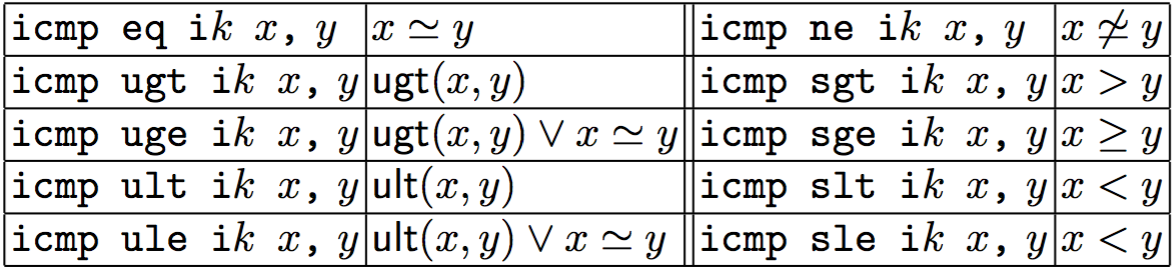
\includegraphics[width=\textwidth]{ins1.png}
\end{figure}

For example,
\footnotesize
\begin{eqnarray}
ugt(x,y) & = & (x \ge 0 \land y \ge 0 \land x > y) \nonumber\\
& & \lor\; (x \ge 0 \land y < 0) \nonumber\\
& & \lor\; (x < 0 \land y < 0 \land x > y) \nonumber
\end{eqnarray}
\end{frame}

\begin{frame}{Phase 1 (cont'd)}
\begin{figure}
  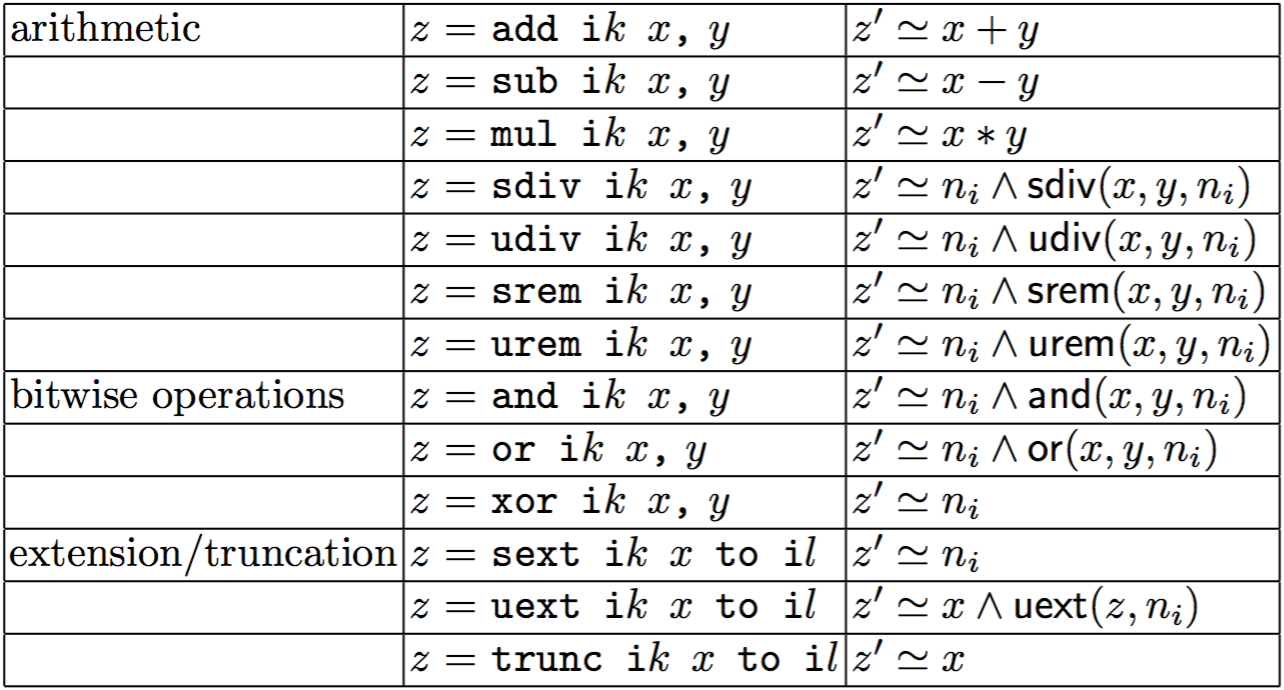
\includegraphics[width=\textwidth]{ins2.png}
\end{figure}
\end{frame}

\begin{frame}[fragile]{Phase 1 (cont'd)}
Some instructions are approximated by introducing new variables and
constraints. 

\medskip
For example, the \verb|and| instruction, its constraint:
\begin{eqnarray}
and(x,y,n_i) & = & (x \ge 0 \land y \ge 0 \land n_i \ge 0 \land n_i \le x \land n_i \le y) \nonumber\\
& & \lor\; (x \ge 0 \land y < 0 \land n_i \ge 0 \land n_i \le x) \nonumber\\
& & \lor\; (x < 0 \land y \ge 0 \land n_i \ge 0 \land n_i \le y) \nonumber\\
& & \lor\; (x < 0 \land y < 0 \land n_i < 0 \land n_i \le x \land n_i \le y) \nonumber
\end{eqnarray}
\end{frame}

\begin{frame}{Phase 2}
Phase 2 is performed after generating the \texttt{int}-based TRS. The
wrap-around behavior of the arithmetical instructions is modeled by
modifying the generated \texttt{int}-based TRS.

For this, the wrap-around behavior is simulated by explicitly
normalizing the resulting integers to be in the appropriate ranges.

Each rewrite rule
\begin{center}
$\rho : f(x_1,\ldots,x_n) \rightarrow g(p_1,\ldots,p_m) ~ \llbracket \varphi \rrbracket$
\end{center}
should be replaced by:
\begin{figure}
  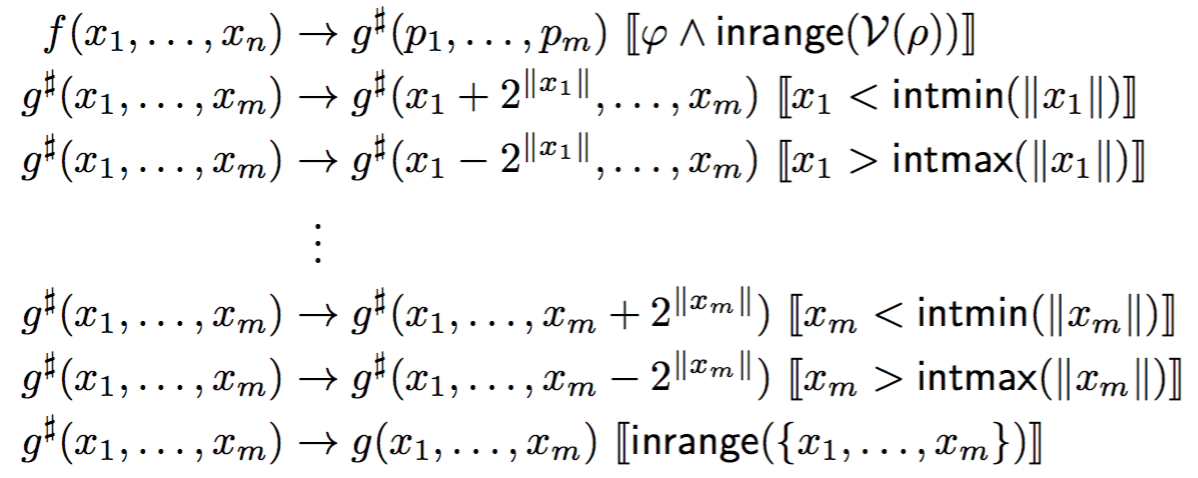
\includegraphics[width=0.6\textwidth]{rules.png}
\end{figure}

\end{frame}

\begin{frame}[fragile]{Phase 2 (cont'd)}
For example, the rule 
\begin{center}
$\verb|bb|(\verb|i.0|) \rightarrow \verb|bb1|(\verb|i.0|) + 1)$
\end{center}
is replaced by
\begin{block}{}
\begin{tabular}{rcl}
$\verb|bb|(\verb|i.0|)$ & $\rightarrow$ 
  & $\verb|bb1|^\#(\verb|i.0| + 1) ~ \llbracket inrange(\verb|i.0|) \rrbracket$ \\
$\verb|bb1|^\#(\verb|i.0|)$ & $\rightarrow$ 
  & $\verb|bb1|^\#(\verb|i.0| + 2^{32}) ~ \llbracket \verb|i.0| < intmin(32) \rrbracket$ \\
$\verb|bb1|^\#(\verb|i.0|)$ & $\rightarrow$ 
  & $\verb|bb1|^\#(\verb|i.0| - 2^{32}) ~ \llbracket \verb|i.0| > intmax(32) \rrbracket$ \\
$\verb|bb1|^\#(\verb|i.0|)$ & $\rightarrow$ 
  & $\verb|bb1|(\verb|i.0|) ~ \llbracket inrange(\verb|i.0|) \rrbracket$ \\
\end{tabular}
\end{block}
\end{frame}

\section{Conclusion}

\begin{frame}{Conclusion}
\begin{itemize}
\item The approach is \emph{sound}.
\begin{itemize}
\item The instructions are \emph{soundly} approximated.
\item The wrap-around behavior is correctly modeled.
\end{itemize}
\item The implementation is powerful than the related approach in
  [CKR+10], with a comparable average time.
\item The approach can be combined with other existing techniques for
  analyzing termination of transition systems/\texttt{int}-based TRSs.
\end{itemize}
\end{frame}

\begin{frame}
\begin{center}
\LARGE Thank you!
\end{center}
\end{frame}

\end{document}
